\documentclass{ieeeaccess}
\usepackage{cite}
\usepackage{amsmath,amssymb,amsfonts}
\usepackage{algorithm}
\usepackage{algorithmicx}
\usepackage{algpseudocode}
%% \usepackage{caption}
\usepackage{graphicx}
\usepackage{textcomp}

\usepackage{bm}

\usepackage{multirow}

% \usepackage{hyperref}

\usepackage{array}
\setlength\extrarowheight{3pt}

\algnewcommand\algorithmicforeach{\textbf{for each}}
\algdef{S}[FOR]{ForEach}[1]{\algorithmicforeach\ #1\ \algorithmicdo}

\providecommand{\e}[1]{\ensuremath{\times 10^{#1}}}

\def\BibTeX{{\rm B\kern-.05em{\sc i\kern-.025em b}\kern-.08em
    T\kern-.1667em\lower.7ex\hbox{E}\kern-.125emX}}

\begin{document}
\history{Date of publication xxxx 00, 0000, date of current version xxxx 00, 0000.}
\doi{10.1109/ACCESS.2017.DOI}

\title{Fuzzy Grade of Membership as a Consensus and Synchronization Mechanism in Cooperative Fuzzy Agent-Based Models}
\author{
    \uppercase{Amaury Hernandez-Aguila\authorrefmark{1},
    Mario Garc\'{i}a-Valdez\authorrefmark{1},
    Juan-Juli\'{A}n Merelo-Guerv\'{o}s\authorrefmark{2},
    Manuel Casta\~{n}\'{o}n-Puga\authorrefmark{3} and
    Oscar Castillo L\'{o}pez\authorrefmark{1}}}
\address[1]{National Technological Institute of Mexico, Calzada Del Tecnol\'{o}gico s/n, Fraccionamiento Tomas Aquino, Tijuana, BC 22414 Mexico (e-mail: {amerhag,mario,ocastillo}@tectijuana.edu.mx)}
\address[2]{University of Granada, Campus Aynadamar Daniel Saucedo Aranda s/n, Granada 18071, 80523 Spain (e-mail: jmerelo@geneura.ugr.es)}
\address[3]{Autonomous University of Baja California, Calzada Universidad 14418, Tijuana, BC, 22390, Mexico (e-mail: puga@uabc.edu.mx)}

\tfootnote{}

\markboth
{Author \headeretal: Preparation of Papers for IEEE TRANSACTIONS and JOURNALS}
{Author \headeretal: Preparation of Papers for IEEE TRANSACTIONS and JOURNALS}

\corresp{Corresponding author: Mario Garc\'{i}a-Valdez (e-mail: mario@tectijuana.edu.mx).}

\begin{abstract}

\end{abstract}
\begin{keywords}
% Check keywords from here:
% http://www.ieee.org/organizations/pubs/ani_prod/keywrd98.txt
  Economic forecasting, fuzzy systems, multi-agent system, activation function, forex market.
\end{keywords}

\titlepgskip=-15pt

\maketitle

\section{Introduction}
\label{section:introduction}

One of the challenges in multi-agent systems is the implementation of
a coordination control mechanism that manages the agents in a model to
collaboratively reach their goals. This challenge can be dissected
into multiple sub-challenges, which include consensus and
synchronization among the agents \cite{dorri2018multi}. Reaching a
consensus among the agents is crucial for obtaining outputs from a
model which take into consideration the state of all of its agents,
while a synchronization mechanism allows heterogeneous agents to take
action when it is appropriate. The method proposed in this paper
addresses


\section{State of the Art}
\label{section:state-of-the-art}


\section{Preliminaries}
\label{section:preliminaries}
\section{Proposed Method}
\label{section:proposed-method}


\section{Model}
\label{section:model}
\section{Experiments}
\label{section:experiments}
\section{Results}
\label{section:results}
\section{Conclusion}
\label{section:conclusion}
\section{Future Work}
\label{section:future-work}

\section*{Acknowledgment}
This paper has been supported in part by project DeepBio (TIN2017-85727-C4-2-P).

\begin{IEEEbiography}[{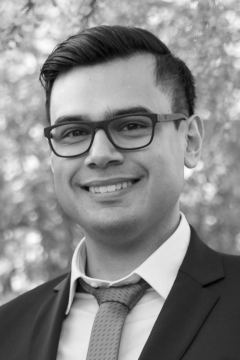
\includegraphics[width=1in,height=1.25in,clip,keepaspectratio]{img/amaury-1by1half-in.png}}]{Amaury
    Hernandez-Aguila}

  Amaury Hernandez-Aguila received the Ph.D degree in Computer Science and the 
  M.Sc. degree in Computer Science from the Tijuana Institute of Technology,
  Mexico, in 2014 and 2019, respectively. He is currently participating in a
  post-doctoral program in Tijuana Institute of Technology, researching how
  multi-agent systems and fuzzy logic can be used for the prediction of
  financial markets.

\end{IEEEbiography}

\begin{IEEEbiography}[{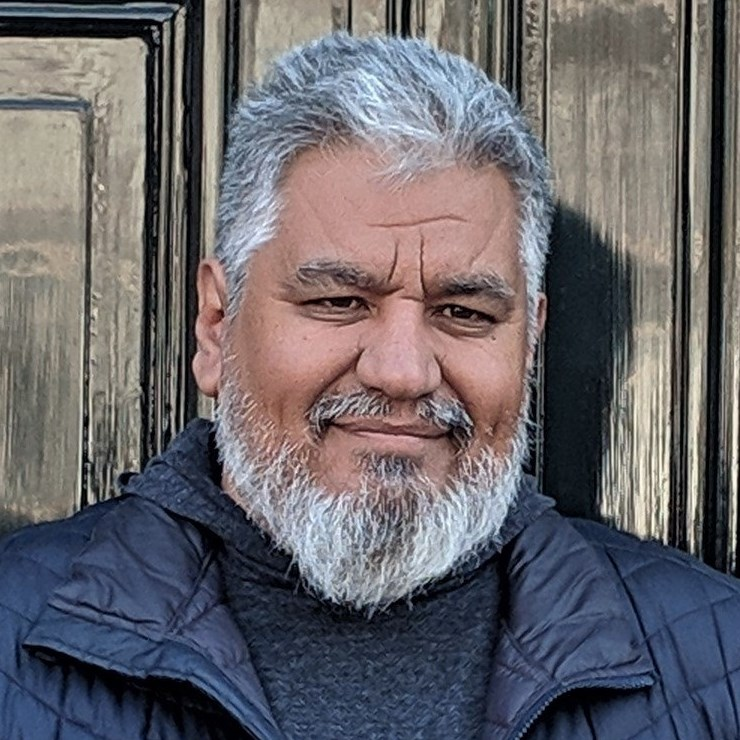
\includegraphics[width=1in,height=1.25in,clip,keepaspectratio]{img/Garcia.jpg}}]{Mario Garc\'{i}a Valdez} 
  Dr. Garc\'{i}a-Valdez is a full-time research professor at the Tijuana
  Institute of Technology. He's interested in the personalization of
  interactive systems, voluntary computing, parallel evolutionary
  computation, interactive evolutionary computation.
\end{IEEEbiography}

\begin{IEEEbiography}[{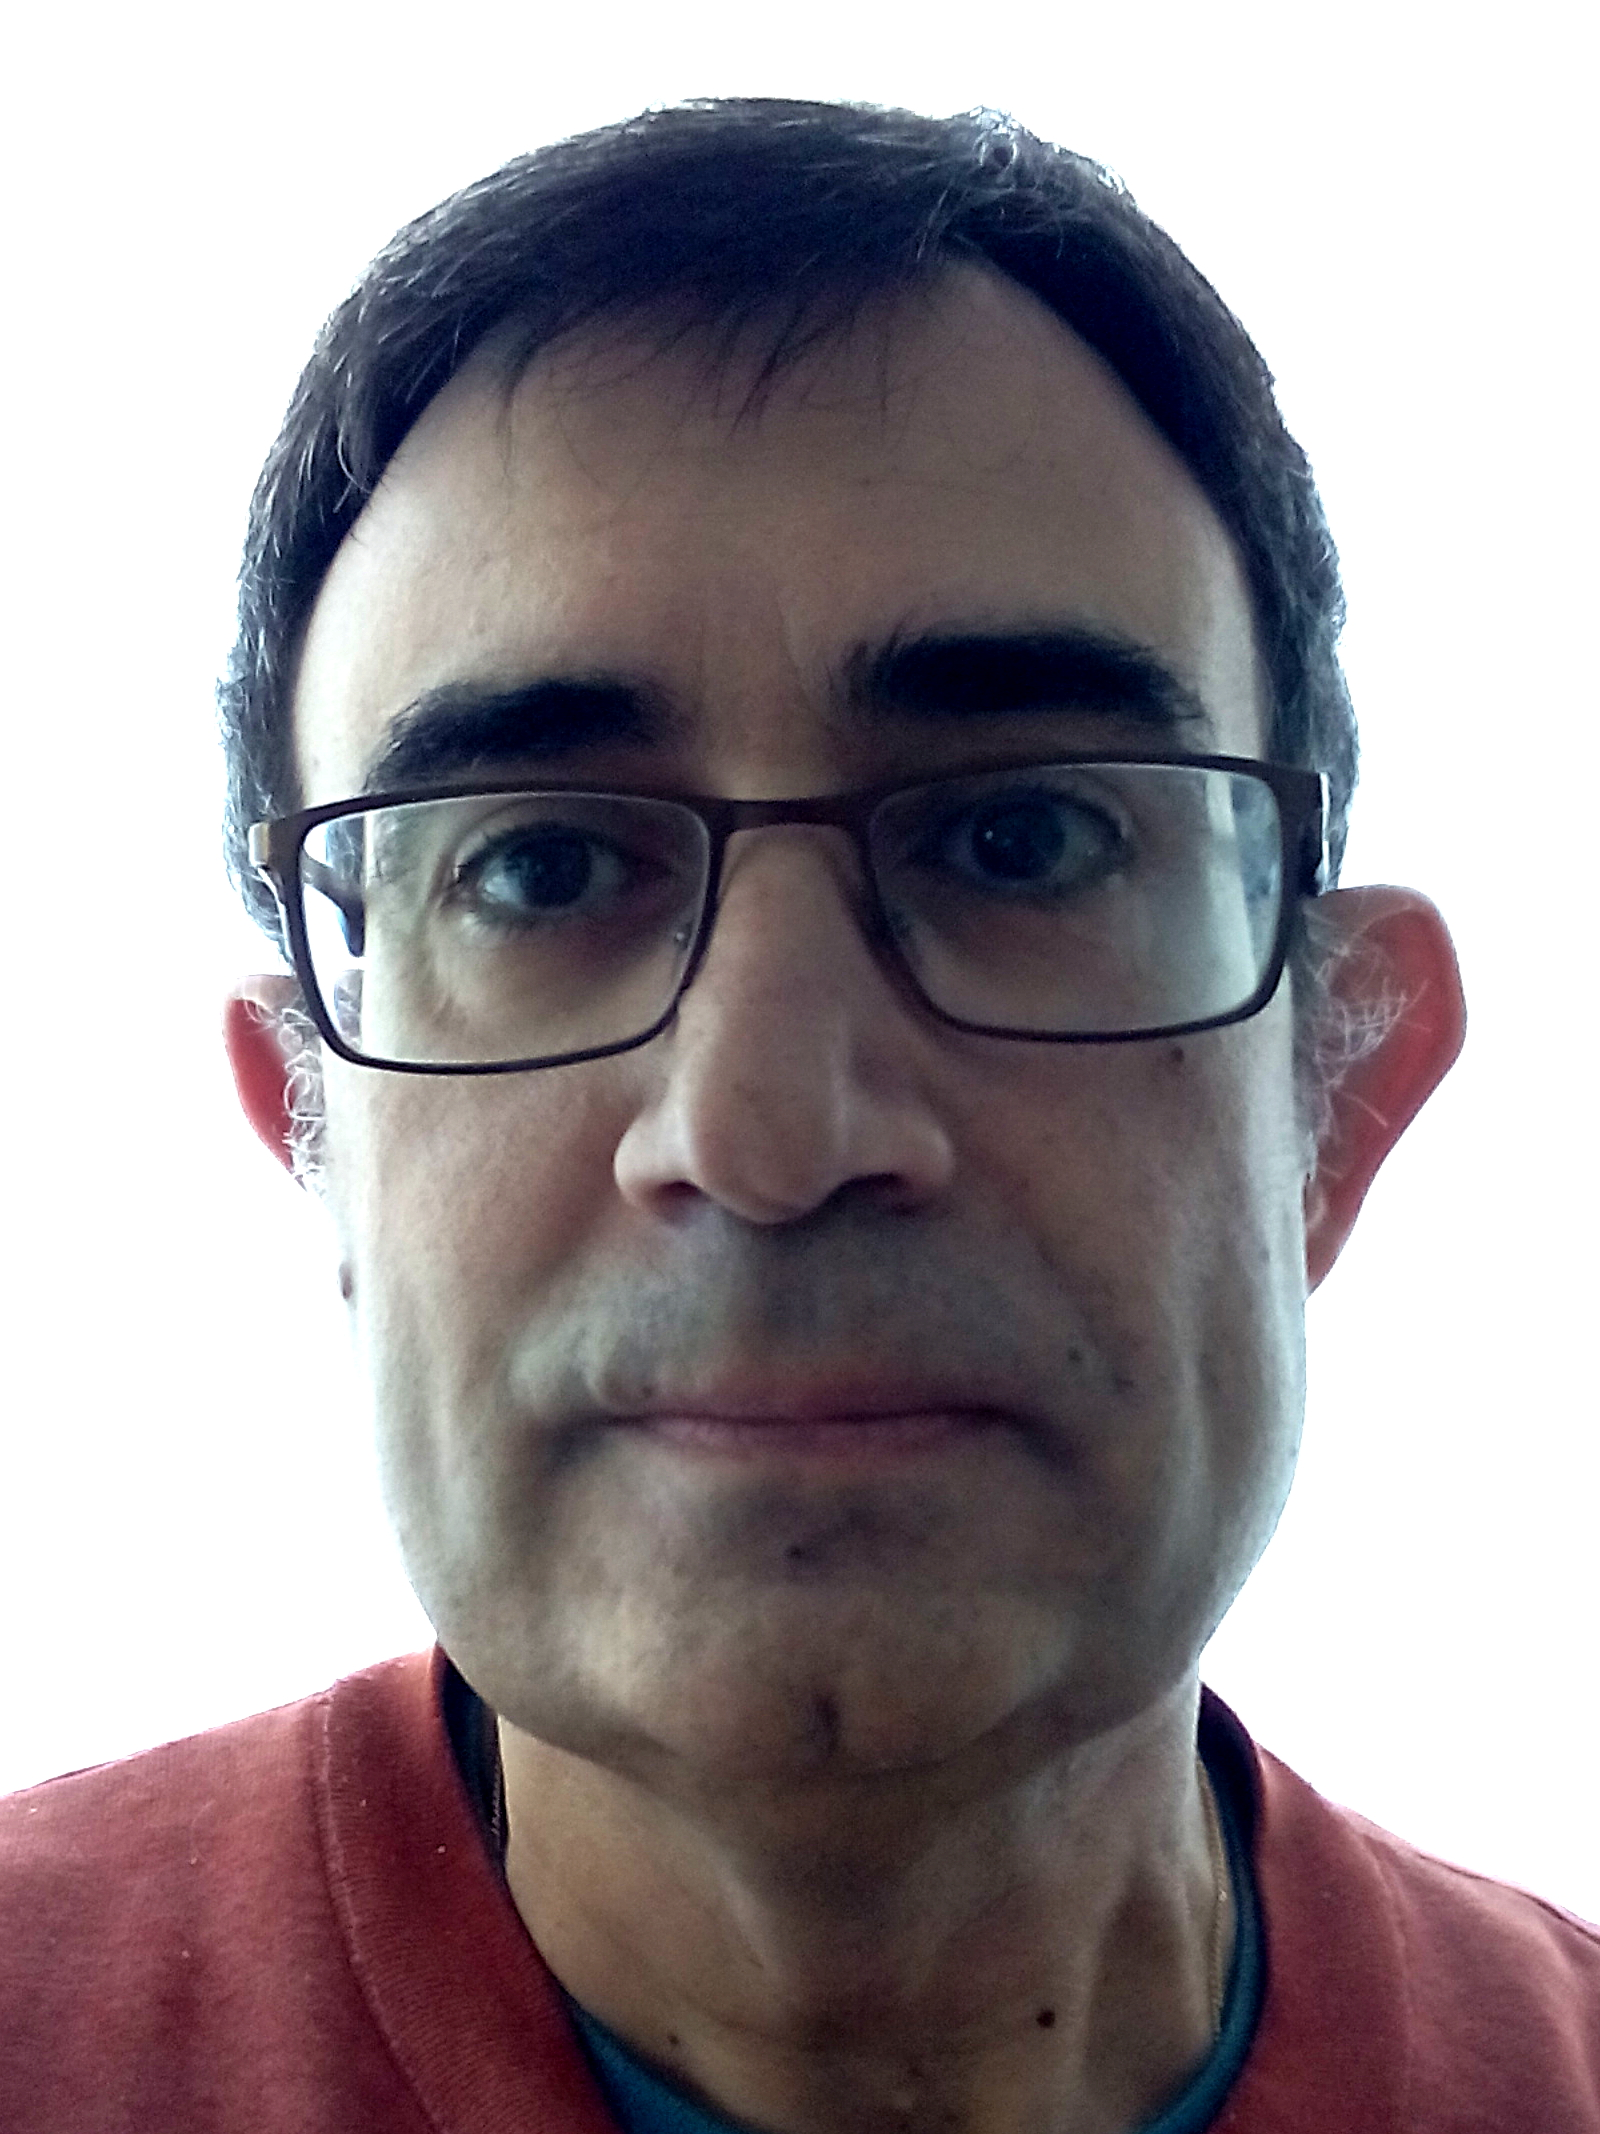
\includegraphics[width=1in,height=1.25in,clip,keepaspectratio]{img/jj-2016-10.jpg}}]{JJ Merelo Guerv\'{o}s} 
  JJ Merelo is professor at the university of Granada, where he obtained a
  degree in Theoretical Physics and a PhD in Physics in 1994. He's mainly
  interested in evolutionary algorithms, open source software and complex
  systems.
  
\end{IEEEbiography}

\begin{IEEEbiography}[{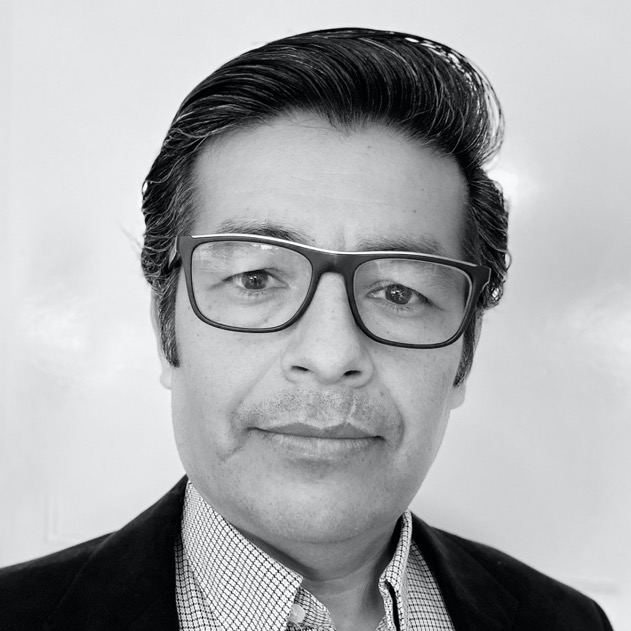
\includegraphics[width=1in,height=1.25in,clip,keepaspectratio]{img/Puga.jpg}}]{Manuel
    Casta\~{n}\'{o}n Puga} Manuel Casta\~{n}\'{o}n-Puga is Professor at Autonomous University of
  Baja California. He obtained a PhD on Computer Sciences from Autonomous
  University of Baja California in Mexico, and a Masters on Computer Sciences and
  Bachelor in Engineering at Tijuana Technology Institute, in his native Tijuana,
  Mexico. His research of modeling and simulation, agent-base simulation,
  hybrid-intelligent agents and multi-agent systems explores the way in which
  software agents could be used to describe multidimensional environments,
  innovation, evolution and adaptation in complex adaptive systems. Dr.
  Casta\~{n}\'{o}n-Puga collaborates with multidisciplinary researchers and scientists to
  create multidimensional computer simulations of societies, political ideologies,
  trading economies and urban landscapes. His research also intends to incorporate
  the ideas of complexity into the mainstream of engineering and in particular to
  its instruction at the undergraduate level. \end{IEEEbiography}


\begin{IEEEbiography}[{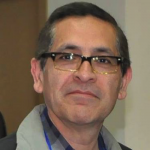
\includegraphics[width=1in,height=1.25in,clip,keepaspectratio]{img/Castillo.png}}]{Oscar
    Castillo L\'{o}pez} Oscar Castillo holds the Doctor in Science degree (Doctor
  Habilitatus) in Computer Science from the Polish Academy of Sciences.
  He is a Professor of Computer Science in the Graduate Division, Tijuana
  Institute of Technology, Tijuana, Mexico. In addition, he is serving as Research
  Director of Computer Science and head of the research group on Hybrid Fuzzy
  Intelligent Systems. Currently, he is President of HAFSA (Hispanic American
  Fuzzy Systems Association) and Past President of IFSA (International Fuzzy
  Systems Association). Prof. Castillo is also Chair of the Mexican Chapter of the
  Computational Intelligence Society (IEEE). He also belongs to the Technical
  Committee on Fuzzy Systems of IEEE and to the Task Force on ``Extensions to
  Type-1 Fuzzy Systems''. He is currently Associate Editor of the Information
  Sciences Journal, Applied Soft Computing Journal, Journal of Engineering
  Applications on Artificial Intelligence, Granular Computing Journal and the
  International Journal of Fuzzy Systems. Finally, he recently received the Recognition as
  Highly Cited Researcher in 2017 and 2018 by Clarivate Analytics and Web of
  Science \end{IEEEbiography}

\bibliography{bibliography}
\bibliographystyle{IEEEtran}

\EOD

\end{document}
